\section{Detecting slower workers in workers}
    \subsection{First to finish application}
        Next, we provide a synthetic application modeling an application that can be modeled by a first to finish operator

        \paragraph{Why first to finish?} Recall the previous FTF graph \cref{fig:ftf}. Assume a send request to "the cloud" that waits for a response or a timeout, it is modeled by a FTF operator. 
       \subsubsection{Using the wrong operator}
            What happens if the wrong operator is chosen to represent the causal relationships between the outcomes? What if the user believes that the system diagram is the one we presented before \cref{fig:mm1k}? The result on the oscilloscope will clearly show that something is wrong! 
            \begin{figure}[H]
                \centering
                \begin{subfigure}{.5\textwidth}
                    \centering
                    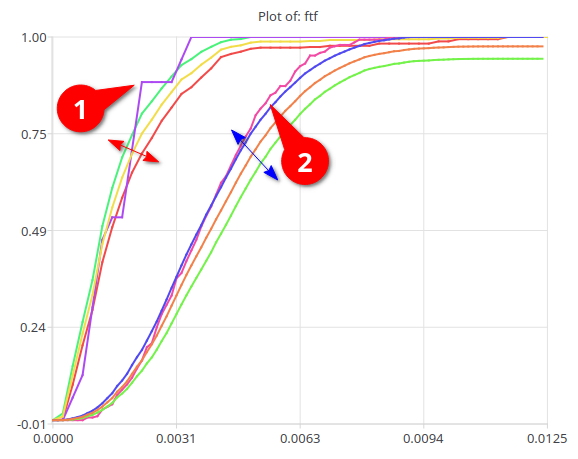
\includegraphics[width =0.98\textwidth]{img/bad1.png}
                    \label{fig:bad}
                \end{subfigure}%
                \begin{subfigure}{.5\textwidth}%
                    \centering%
                    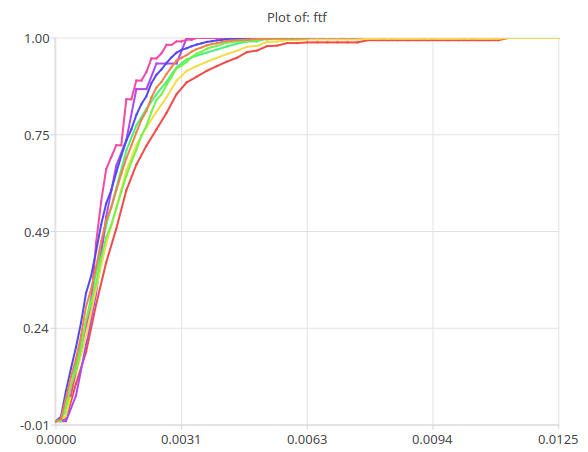
\includegraphics[width =0.98\textwidth]{img/good.png}%
                    \label{fig:good}%
                \end{subfigure}%
                \caption{\textit{(Left)} FTF plot \textbf{with wrong outcome diagram definition} as shown in the oscilloscope. (1) Observed $\Delta$Q. (2) Calculated $\Delta$Q. \\
                \textit{(Right)} FTF plot \textbf{with correct outcome diagram definition} as shown in the oscilloscope. Observed $\Delta$Q and calculated $\Delta$Q overlapping.}
                \label{fig:ftf_osc}%
            \end{figure}%
        On the left, we can observe how the \textbf{calculated $\Delta$Q} (2) is clearly greater than the \textbf{observed $\Delta$Q} (1). A difference this drastic tells us that the proposed outcome diagram does not correctly represent the actual system. On the right, if no dependencies are present and the correct operator is chosen, the two graphs will overlap.

        \subsubsection{Introducing a slower component}
            Let us introduce a slower worker into the system, we introduce an artificial delay into worker\_2 (about 20ms). If the oscilloscope works correctly, the paradigm operations are sound and no dependencies are present in the system, we should not see any difference in the observed and calculated $\Delta$Qs of the FTF operator.

            \begin{figure}[H]
                \centering 
                \begin{subfigure}{.5\textwidth}
                    \centering
                    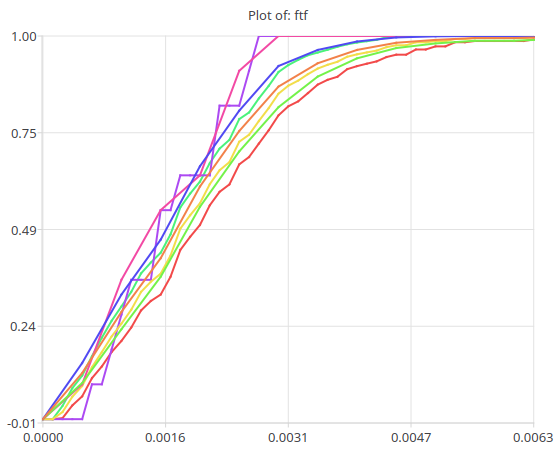
\includegraphics[width =0.98\textwidth]{img/delay31.png}
                    \label{fig:ftf_art_d}
                \end{subfigure}%
                \begin{subfigure}{.5\textwidth}%
                    \centering%
                    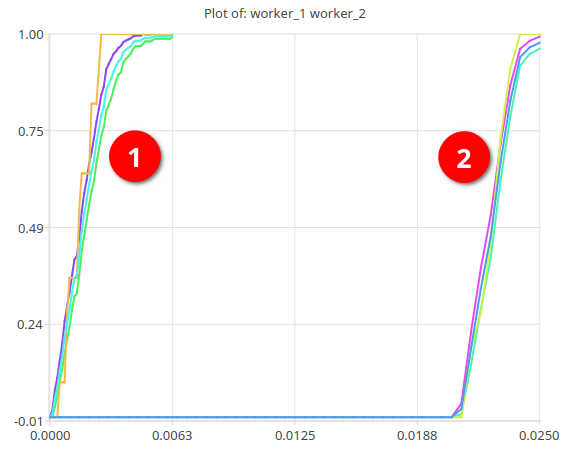
\includegraphics[width =0.98\textwidth]{img/delay32.png}%
                    \label{fig:ftf_art_dw}%
                \end{subfigure}%
                \caption{\textit{(Left)} FTF plot of worker\_1 and worker\_2, observed and calculated $\Delta$Q overlapping.\\
                \textit{(Right)} worker\_1 (1) and worker\_2 (2) $\Delta$Qs. \\
                The FTF plot correctly displays how worker\_2 does not have an effect on the ftf plot.}
                \label{fig:ftf_w1w2}%
            \end{figure}%

